\section{Phenix Molprobity protocol}
\label{app:molprobityProtocol}%a130
Protocol designed to assess the geometry of refined atomic structures without considering electron density maps in \scipion by using $MolProbity$ \citep{davis2004}. Integrated in cryo-EM validation tools of $Phenix$ software suite (\url{https://www.phenix-online.org/}), $MolProbity$ tool validates geometry and dihedral-angle combinations of atomic structures. $MolProbity$ scores can guide the refinement process of the atomic structure to get a good fitting of the atomic structure to the cryo-EM density map. Adding a volume as input in \ttt{Phenix MolProbity} protocol is not mandatory, although if a volume is provided \ttt{Real Space Correlation} coefficients between map and model will be calculated.\\

\begin{itemize}
 \item \scipion menu:\\
  \ttt{Protocols SPA -> Model building} (\ffigure{fig:app_protocol_molprobity_1} (A))\\
  
 \item Protocol form parameters (\ffigure{fig:app_protocol_molprobity_1} (B)):\\
  
    \begin{figure}[H]
     \centering 
     \captionsetup{width=.7\linewidth} 
     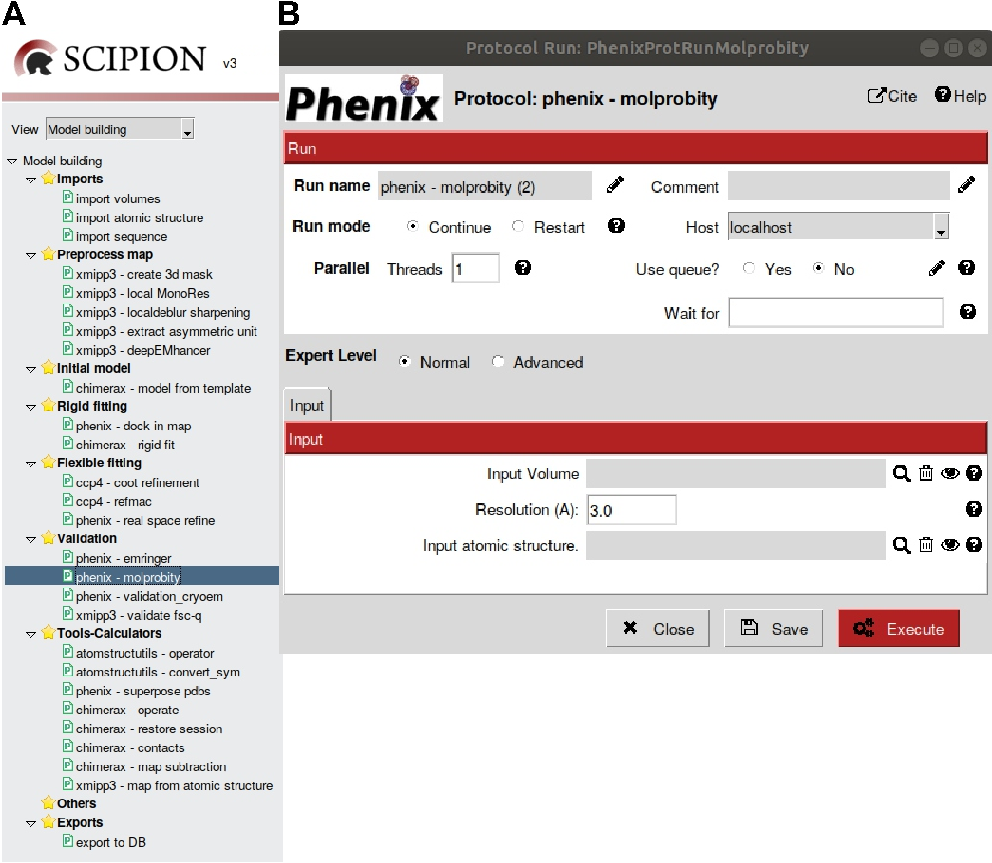
\includegraphics[width=0.90\textwidth]{Images_appendix/Fig143.pdf}
     \caption{Protocol \scommand{phenix - molprobity}. A: Protocol location in \scipion menu. B: Protocol form.}
     \label{fig:app_protocol_molprobity_1}
    \end{figure}

    \begin{itemize}
     \item \ttt{Input Volume}: (Optional) Electron density map previously downloaded or generated in \scipion and fitted to an atomic structure.
     \item \ttt{Resolution (\AA)}: Map resolution when a volume has been selected in the \ttt{Input Volume} parameter.
     \item \ttt{Input atomic structure}: Atomic structure previously downloaded or generated in \scipion and fitted to an electron density map.\
    \end{itemize}
    
 \item Protocol execution:\\
 Adding specific sequence label is recommended in \ttt{Run name} section, at the form top. To add the label, open the protocol form, press the pencil symbol at the right side of \ttt{Run name} box, complete the label in the new opened window, press OK, and finally close the protocol. This label will be shown in the output summary content (see below). If you want to run again this protocol, do not forget to set to \ttt{Restart} the \ttt{Run mode}.\\
  Press the \ttt{Execute} red button at the form bottom.\\
  
 \item Visualization of protocol results:\\
  
  After executing the protocol, press \ttt{Analyze Results} and the results window will be opened (\ffigure{fig:app_protocol_molprobity_2}).\\ 
  
  \begin{figure}[H]
     \centering 
     \captionsetup{width=.7\linewidth} 
     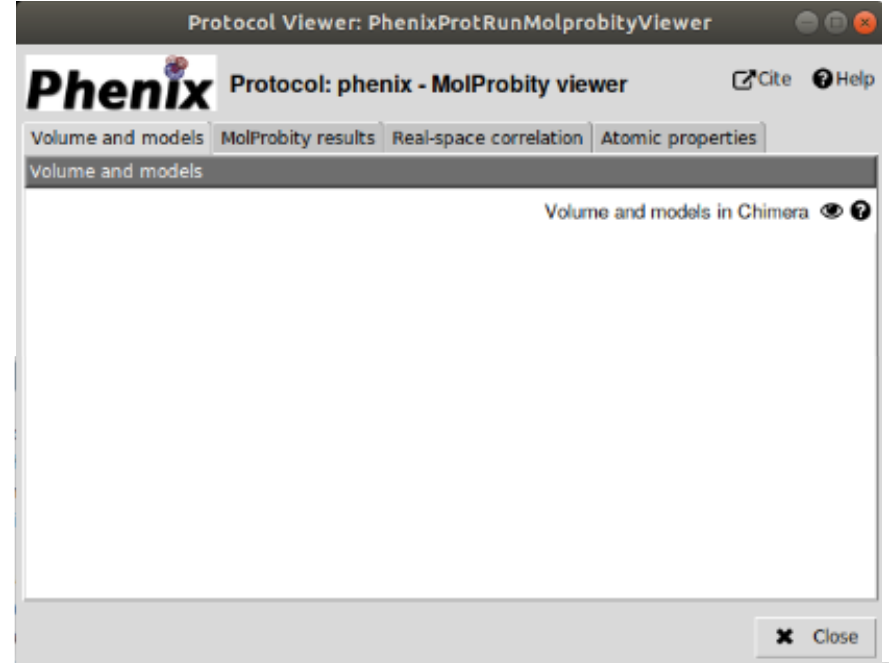
\includegraphics[width=0.60\textwidth]{Images_appendix/Fig144.pdf}
     \caption{Protocol \scommand{phenix - molprobity}. Taps to visualize $MolProbity$  and Real space correlation results.}
     \label{fig:app_protocol_molprobity_2}
    \end{figure}
    
   Four taps are shown in the upper part of the results window:
   \begin{itemize}
     \item XXXX Maps and models:
     \chimera graphics window displays coordinate axes, selected input volume, if it has been provided, and the fitted atomic structure.
     \item XXXX MolProbity Results(\ffigure{fig:app_protocol_molprobity_3}):
        \begin{figure}[H]
         \centering 
         \captionsetup{width=.7\linewidth} 
         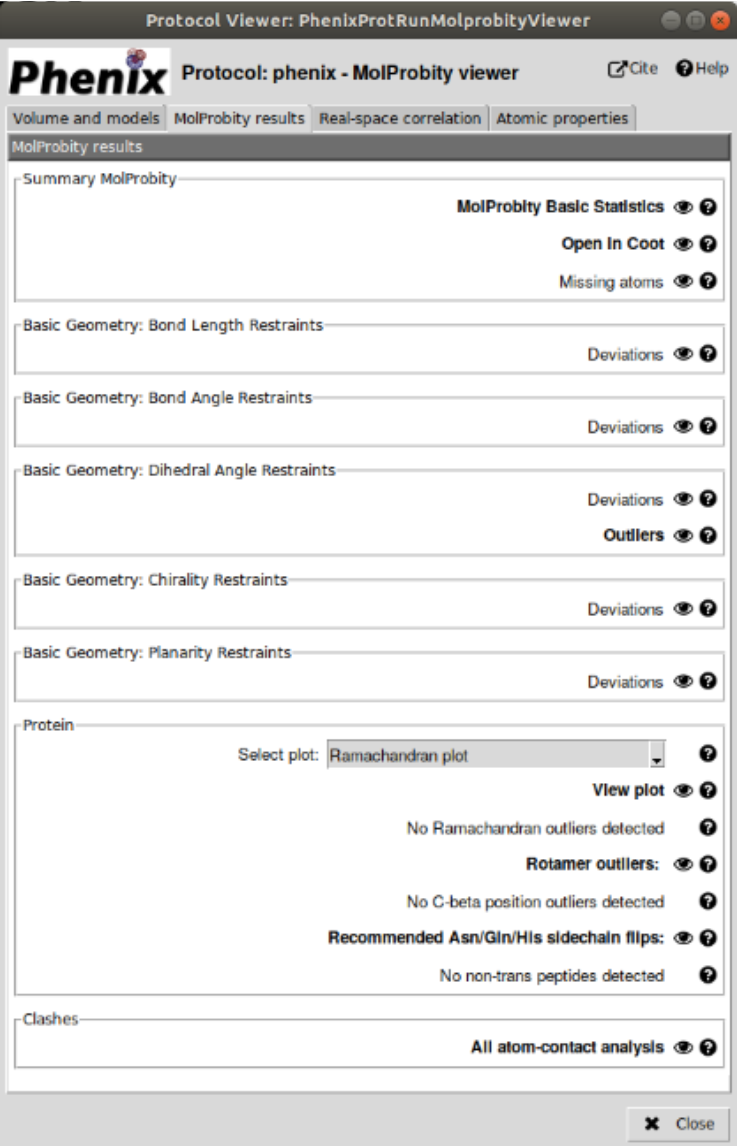
\includegraphics[width=0.80\textwidth]{Images_appendix/Fig145.pdf}
         \caption{Protocol \scommand{phenix - molprobity}. $MolProbity$ results.}
         \label{fig:app_protocol_molprobity_3}
        \end{figure}
      \begin{itemize}
        \item XXX Results table:
        
        \begin{figure}[H]
         \centering 
         \captionsetup{width=.7\linewidth} 
         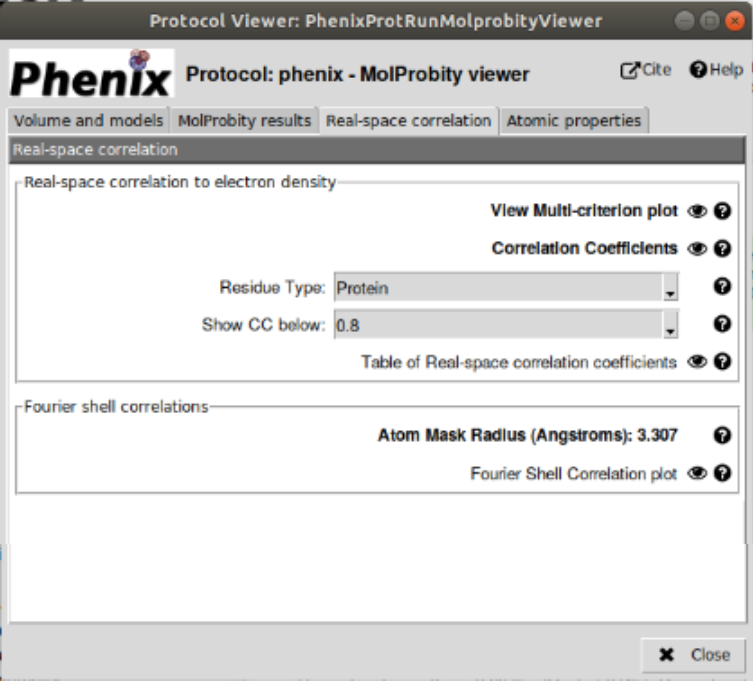
\includegraphics[width=0.80\textwidth]{Images_appendix/Fig146.pdf}
         \caption{Protocol \scommand{phenix - molprobity}. Real space correlation results.}
         \label{fig:app_protocol_molprobity_4}
        \end{figure}
         \begin{itemize}
          
          
         \end{itemize}

        \item XXX Thresholds Scan:
         \begin{itemize}
          \item Plot of EMRinger Score and Percentage of Rotameric Residues regarding Electron Potential Threshold.
         \end{itemize}
        \item XXXX
      \end{itemize}
    \end{itemize}
    
 \item Summary content:\\
 
  \ttt{SUMMARY} box:\\Statistics included in the above Final Results Table (an example can be seen in \ffigure{fig:molprobity_protocol} (7).

\end{itemize}
